%\VignetteIndexEntry{Data and analysis in phylotools}
%\VignetteDepends{phylotools, ape, picante, seqRFLP}
%\VignettePackage{phylotools}
\documentclass[12pt]{article}
\usepackage{amssymb,amsmath}
\usepackage{geometry}
\geometry{letterpaper}
\usepackage{graphicx}
\usepackage{url}


\title{An introduction to the phylotools package}
\author{ Jinlong Zhang, Xiangcheng Mi, Nancai Pei}

\date{Oct 2010}
\usepackage{Sweave}
\begin{document}



\maketitle

\tableofcontents

\section{Introduction}

"phylotools" is an R package for construction of "supermatrix" which will be used in the further analysis of phylogenies from DNA barcoding sequences. It is primary designed for creat supermatrix more easily in R. See Kress et al. 2010 for further information.
The slashes at both ends of one sequence in the aligned sequences will be replaced by "?", the ones at the internal parts of the sequences will be retained. 


\section{How to install phylotools}

The \texttt{phylotools} is available at CRAN mirror \url{http://cran.r-project.org/web/packages/}. To install the package, just type "\texttt{install.packages("phylotools")}".
The R will automatically download and install the package. Once it is installed, users have to type it can be loaded by typing:

\begin{Schunk}
\begin{Sinput}
> library(phylotools)
\end{Sinput}
\end{Schunk}



\section{Data Input}
User have to provide the aligned sequences in phylip format. Sequences from the same species must have the same name in different phylip files. For example: the sequences from \texttt{Ulmus pumila}, should have have same name in different alinment files. These files maybe generated by the software for sequence alignments, for example: ClustalW, ClustaX, MUSCLE.

\section{Data Output}
Output is a super matrix with unknown sites represent by "?". See Tabel 1 for detail.
In order to build the supermatrix, users have to provide the files listed as follow.. 
(1)  One file for rbcLa, in phylip format
(2)  One file for matK, in phylip format.
(3)  Files for trnH-psbA aligned sequences. The trnH-psbA sequences evolve much more rapidly and often aligned by species in on order or even family. Users for realy data may have tens of trnH-psbA aligned files in phylip format.

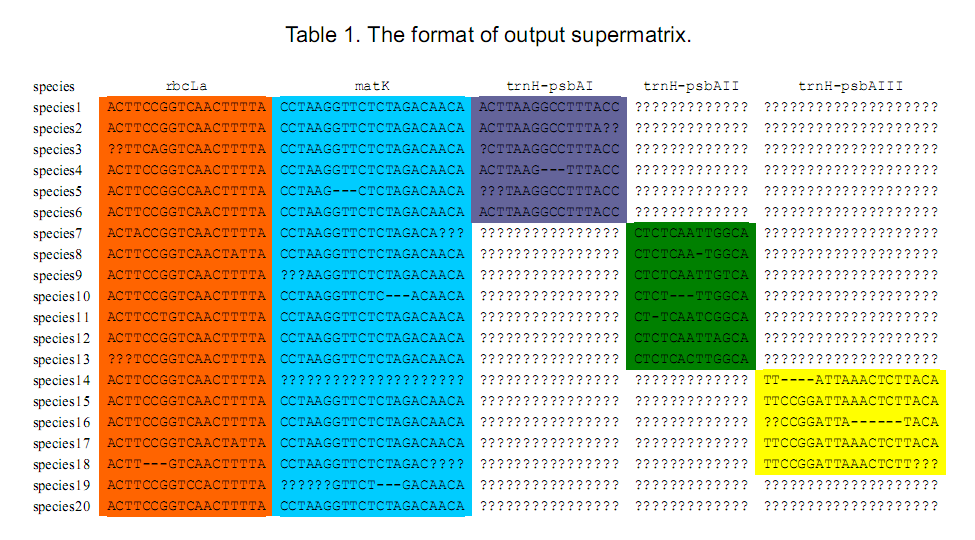
\includegraphics[width = 15cm]{table1.PNG}

\section{Step by step guide building a supermatrix}
Assume we have the aligned files in phylip format named :

"\texttt{rbcla.phy}", 
"\texttt{matK.phy}", 
"\texttt{trn1.phy}","\texttt{trn2.phy}", "\texttt{trn3.phy}", "\texttt{trn4.phy}"

Users may follow the steps to build the supermatrix and save the results to file:

\subsection{Step 1: Copy the phy files to working directory}
 Copy ALL the .phy files to the same directory. Here we use the data provided in the package in directory "extdata" 
 
\subsection{Step 2 Set working directory}
type the following command to set the working directory the files exists.

\begin{Schunk}
\begin{Sinput}
> dir <- system.file("extdata", package = "phylotools")
> setwd(dir)
\end{Sinput}
\end{Schunk}

\subsection{Step 3 Build supermatrix using supermat}
Use the function "\texttt{supermat()}" to build a "super" matrix representing the relationships between the sequences. Type:

\begin{Schunk}
\begin{Sinput}
> supermat <- supermat(rbcl = "rbcla.phy", matk = "matK.phy", 
+     trn = c("trn1.phy", "trn2.phy", "trn3.phy", "trn4.phy"))
\end{Sinput}
\end{Schunk}
	  
\subsection{Step 4 Save the supermatrix to a Phylip file}
Save the supermatrix to file 

\begin{Schunk}
\begin{Sinput}
> write.mat(supermat, "result.phy")
\end{Sinput}
\end{Schunk}

\section{Literature cited}

\begin{itemize}
\item{Kress W., Erickson D., Jones F., Swenson N., Perez R., Sanjur O., Bermingham E., Plant DNA barcodes and community phylogeny of a tropical forest dynamics plot in Panama. Proceedings of the National Academy of Sciences of the United States of America. 2009 18621-18626 }
\end{itemize}

\end{document}
